\documentclass[twoside]{book}

% Packages required by doxygen
\usepackage{fixltx2e}
\usepackage{calc}
\usepackage{doxygen}
\usepackage[export]{adjustbox} % also loads graphicx
\usepackage{graphicx}
\usepackage[utf8]{inputenc}
\usepackage{makeidx}
\usepackage{multicol}
\usepackage{multirow}
\PassOptionsToPackage{warn}{textcomp}
\usepackage{textcomp}
\usepackage[nointegrals]{wasysym}
\usepackage[table]{xcolor}

% Font selection
\usepackage[T1]{fontenc}
\usepackage[scaled=.90]{helvet}
\usepackage{courier}
\usepackage{amssymb}
\usepackage{sectsty}
\renewcommand{\familydefault}{\sfdefault}
\allsectionsfont{%
  \fontseries{bc}\selectfont%
  \color{darkgray}%
}
\renewcommand{\DoxyLabelFont}{%
  \fontseries{bc}\selectfont%
  \color{darkgray}%
}
\newcommand{\+}{\discretionary{\mbox{\scriptsize$\hookleftarrow$}}{}{}}

% Page & text layout
\usepackage{geometry}
\geometry{%
  a4paper,%
  top=2.5cm,%
  bottom=2.5cm,%
  left=2.5cm,%
  right=2.5cm%
}
\tolerance=750
\hfuzz=15pt
\hbadness=750
\setlength{\emergencystretch}{15pt}
\setlength{\parindent}{0cm}
\setlength{\parskip}{3ex plus 2ex minus 2ex}
\makeatletter
\renewcommand{\paragraph}{%
  \@startsection{paragraph}{4}{0ex}{-1.0ex}{1.0ex}{%
    \normalfont\normalsize\bfseries\SS@parafont%
  }%
}
\renewcommand{\subparagraph}{%
  \@startsection{subparagraph}{5}{0ex}{-1.0ex}{1.0ex}{%
    \normalfont\normalsize\bfseries\SS@subparafont%
  }%
}
\makeatother

% Headers & footers
\usepackage{fancyhdr}
\pagestyle{fancyplain}
\fancyhead[LE]{\fancyplain{}{\bfseries\thepage}}
\fancyhead[CE]{\fancyplain{}{}}
\fancyhead[RE]{\fancyplain{}{\bfseries\leftmark}}
\fancyhead[LO]{\fancyplain{}{\bfseries\rightmark}}
\fancyhead[CO]{\fancyplain{}{}}
\fancyhead[RO]{\fancyplain{}{\bfseries\thepage}}
\fancyfoot[LE]{\fancyplain{}{}}
\fancyfoot[CE]{\fancyplain{}{}}
\fancyfoot[RE]{\fancyplain{}{\bfseries\scriptsize Generated by Doxygen }}
\fancyfoot[LO]{\fancyplain{}{\bfseries\scriptsize Generated by Doxygen }}
\fancyfoot[CO]{\fancyplain{}{}}
\fancyfoot[RO]{\fancyplain{}{}}
\renewcommand{\footrulewidth}{0.4pt}
\renewcommand{\chaptermark}[1]{%
  \markboth{#1}{}%
}
\renewcommand{\sectionmark}[1]{%
  \markright{\thesection\ #1}%
}

% Indices & bibliography
\usepackage{natbib}
\usepackage[titles]{tocloft}
\setcounter{tocdepth}{3}
\setcounter{secnumdepth}{5}
\makeindex

% Hyperlinks (required, but should be loaded last)
\usepackage{ifpdf}
\ifpdf
  \usepackage[pdftex,pagebackref=true]{hyperref}
\else
  \usepackage[ps2pdf,pagebackref=true]{hyperref}
\fi
\hypersetup{%
  colorlinks=true,%
  linkcolor=blue,%
  citecolor=blue,%
  unicode%
}

% Custom commands
\newcommand{\clearemptydoublepage}{%
  \newpage{\pagestyle{empty}\cleardoublepage}%
}

\usepackage{caption}
\captionsetup{labelsep=space,justification=centering,font={bf},singlelinecheck=off,skip=4pt,position=top}

%===== C O N T E N T S =====

\begin{document}

% Titlepage & ToC
\hypersetup{pageanchor=false,
             bookmarksnumbered=true,
             pdfencoding=unicode
            }
\pagenumbering{roman}
\begin{titlepage}
\vspace*{7cm}
\begin{center}%
{\Large My Project }\\
\vspace*{1cm}
{\large Generated by Doxygen 1.8.11}\\
\end{center}
\end{titlepage}
\clearemptydoublepage
\tableofcontents
\clearemptydoublepage
\pagenumbering{arabic}
\hypersetup{pageanchor=true}

%--- Begin generated contents ---
\chapter{Class Index}
\section{Class List}
Here are the classes, structs, unions and interfaces with brief descriptions\+:\begin{DoxyCompactList}
\item\contentsline{section}{\hyperlink{structnode}{node} }{\pageref{structnode}}{}
\item\contentsline{section}{\hyperlink{structnode1}{node1} }{\pageref{structnode1}}{}
\item\contentsline{section}{\hyperlink{structnode__info}{node\+\_\+info} }{\pageref{structnode__info}}{}
\end{DoxyCompactList}

\chapter{File Index}
\section{File List}
Here is a list of all files with brief descriptions\+:\begin{DoxyCompactList}
\item\contentsline{section}{\hyperlink{Lab1_8c}{Lab1.\+c} }{\pageref{Lab1_8c}}{}
\end{DoxyCompactList}

\chapter{Class Documentation}
\hypertarget{classCMatrix}{}\section{C\+Matrix Class Reference}
\label{classCMatrix}\index{C\+Matrix@{C\+Matrix}}
\subsection*{Public Member Functions}
\begin{DoxyCompactItemize}
\item 
\hyperlink{classCMatrix_a768f915421b966dfe28fe346ba262ce7}{C\+Matrix} (const char $\ast$name, int rows, int cols)
\item 
\hyperlink{classCMatrix_a81e958550021cc7a00fda22a46c774f3}{C\+Matrix} (const \hyperlink{classCMatrix}{C\+Matrix} \&other)
\item 
\hyperlink{classCMatrix_aff1a3524e09b0329286c5e231c3f1afb}{$\sim$\+C\+Matrix} ()
\item 
void \hyperlink{classCMatrix_a7878287aa7b5a1404980ff08d3cfeb16}{Set\+Name} (const char $\ast$name)
\item 
const char $\ast$ \hyperlink{classCMatrix_ae6df44c34368fbad7a5bfbda879af3ee}{Get\+Name} () const 
\item 
void \hyperlink{classCMatrix_af90c46bd02b2a57c58ffcff64d8dd3c6}{Get\+Input} ()
\item 
void \hyperlink{classCMatrix_afd8bcbf3b820b37223886632251e4d55}{Fill\+Simulated\+Input} ()
\item 
double \hyperlink{classCMatrix_a865ff8f610be372e666fbf24d5b73a3a}{Determinant} ()
\item 
\hyperlink{classCMatrix}{C\+Matrix} \& \hyperlink{classCMatrix_a939d852e81803eddaac29d96d0a1ef84}{operator=} (const \hyperlink{classCMatrix}{C\+Matrix} \&other)
\item 
\hyperlink{classCMatrix}{C\+Matrix} \hyperlink{classCMatrix_acc5e18f7dac42418762e92ebd8d10840}{Co\+Factor} ()
\item 
\hyperlink{classCMatrix}{C\+Matrix} \hyperlink{classCMatrix_a029eef7850029d78359ba09607cd8457}{Adjoint} ()
\item 
\hyperlink{classCMatrix}{C\+Matrix} \hyperlink{classCMatrix_ab8e853a7df8e23889ab233523324ff29}{Transpose} ()
\item 
\hyperlink{classCMatrix}{C\+Matrix} \hyperlink{classCMatrix_abd58298df23c98b8675a81a70c6f140b}{Inverse} ()
\item 
\hyperlink{classCMatrix}{C\+Matrix} \hyperlink{classCMatrix_a0fac0198450dcbcd402e1802dd6b8008}{operator+} (const \hyperlink{classCMatrix}{C\+Matrix} \&other)
\item 
\hyperlink{classCMatrix}{C\+Matrix} \hyperlink{classCMatrix_a26d893cfb384a7c23f5c2c959fe74293}{operator-\/} (const \hyperlink{classCMatrix}{C\+Matrix} \&other)
\item 
\hyperlink{classCMatrix}{C\+Matrix} \hyperlink{classCMatrix_a665fdcc1fda1a9a23e6128f1ec31cc69}{operator$\ast$} (const \hyperlink{classCMatrix}{C\+Matrix} \&other)
\item 
bool \hyperlink{classCMatrix_a2f26b64fa654512fe2a4e954f18e1f1c}{operator==} (const \hyperlink{classCMatrix}{C\+Matrix} \&other)
\end{DoxyCompactItemize}
\subsection*{Public Attributes}
\begin{DoxyCompactItemize}
\item 
double $\ast$$\ast$ \hyperlink{classCMatrix_ab0f18d68cad9b6d750d05a96b60a759d}{m\+\_\+p\+Data}
\end{DoxyCompactItemize}
\subsection*{Private Member Functions}
\begin{DoxyCompactItemize}
\item 
\hyperlink{classCMatrix_a720aa6a48296f4414ac7f9021bc420c4}{C\+Matrix} ()
\end{DoxyCompactItemize}
\subsection*{Private Attributes}
\begin{DoxyCompactItemize}
\item 
int \hyperlink{classCMatrix_ae23e5f8016ba06cfd1cce364a99f5037}{m\+\_\+rows}
\item 
int \hyperlink{classCMatrix_a723f752208c055093012984eaddb62d3}{m\+\_\+cols}
\item 
char \hyperlink{classCMatrix_aecd316cc4360014e817f7dc763aaa957}{m\+\_\+name} \mbox{[}128\mbox{]}
\end{DoxyCompactItemize}
\subsection*{Friends}
\begin{DoxyCompactItemize}
\item 
std\+::istream \& \hyperlink{classCMatrix_a775d8b5122da5b9fdea41520953a4237}{operator$>$$>$} (std\+::istream \&is, \hyperlink{classCMatrix}{C\+Matrix} \&m)
\item 
std\+::ostream \& \hyperlink{classCMatrix_a62d7be0784c5982bf356f96493281902}{operator$<$$<$} (std\+::ostream \&os, const \hyperlink{classCMatrix}{C\+Matrix} \&m)
\end{DoxyCompactItemize}


\subsection{Constructor \& Destructor Documentation}
\index{C\+Matrix@{C\+Matrix}!C\+Matrix@{C\+Matrix}}
\index{C\+Matrix@{C\+Matrix}!C\+Matrix@{C\+Matrix}}
\subsubsection[{\texorpdfstring{C\+Matrix()}{CMatrix()}}]{\setlength{\rightskip}{0pt plus 5cm}C\+Matrix\+::\+C\+Matrix (
\begin{DoxyParamCaption}
{}
\end{DoxyParamCaption}
)\hspace{0.3cm}{\ttfamily [private]}}\hypertarget{classCMatrix_a720aa6a48296f4414ac7f9021bc420c4}{}\label{classCMatrix_a720aa6a48296f4414ac7f9021bc420c4}
\index{C\+Matrix@{C\+Matrix}!C\+Matrix@{C\+Matrix}}
\index{C\+Matrix@{C\+Matrix}!C\+Matrix@{C\+Matrix}}
\subsubsection[{\texorpdfstring{C\+Matrix(const char $\ast$name, int rows, int cols)}{CMatrix(const char *name, int rows, int cols)}}]{\setlength{\rightskip}{0pt plus 5cm}C\+Matrix\+::\+C\+Matrix (
\begin{DoxyParamCaption}
\item[{const char $\ast$}]{name, }
\item[{int}]{rows, }
\item[{int}]{cols}
\end{DoxyParamCaption}
)\hspace{0.3cm}{\ttfamily [inline]}}\hypertarget{classCMatrix_a768f915421b966dfe28fe346ba262ce7}{}\label{classCMatrix_a768f915421b966dfe28fe346ba262ce7}

\begin{DoxyCode}
18                                                       :
19             \hyperlink{classCMatrix_ae23e5f8016ba06cfd1cce364a99f5037}{m\_rows}(rows), \hyperlink{classCMatrix_a723f752208c055093012984eaddb62d3}{m\_cols}(cols)
20         \{
21             strcpy(\hyperlink{classCMatrix_aecd316cc4360014e817f7dc763aaa957}{m\_name}, name);
22             \hyperlink{classCMatrix_ab0f18d68cad9b6d750d05a96b60a759d}{m\_pData} = \textcolor{keyword}{new} \textcolor{keywordtype}{double}*[\hyperlink{classCMatrix_ae23e5f8016ba06cfd1cce364a99f5037}{m\_rows}];
23             \textcolor{keywordflow}{for} (\textcolor{keywordtype}{int} i = 0; i < \hyperlink{classCMatrix_ae23e5f8016ba06cfd1cce364a99f5037}{m\_rows}; i++)
24                 \hyperlink{classCMatrix_ab0f18d68cad9b6d750d05a96b60a759d}{m\_pData}[i] = \textcolor{keyword}{new} \textcolor{keywordtype}{double}[\hyperlink{classCMatrix_a723f752208c055093012984eaddb62d3}{m\_cols}];
25             \textcolor{keywordflow}{for} (\textcolor{keywordtype}{int} i = 0; i < \hyperlink{classCMatrix_ae23e5f8016ba06cfd1cce364a99f5037}{m\_rows}; i++)
26             \{
27                 \textcolor{keywordflow}{for} (\textcolor{keywordtype}{int} j = 0; j < \hyperlink{classCMatrix_a723f752208c055093012984eaddb62d3}{m\_cols}; j++)
28                 \{
29                     \hyperlink{classCMatrix_ab0f18d68cad9b6d750d05a96b60a759d}{m\_pData}[i][j] = 0.0;
30                 \}
31             \}
32         \}
\end{DoxyCode}
\index{C\+Matrix@{C\+Matrix}!C\+Matrix@{C\+Matrix}}
\index{C\+Matrix@{C\+Matrix}!C\+Matrix@{C\+Matrix}}
\subsubsection[{\texorpdfstring{C\+Matrix(const C\+Matrix \&other)}{CMatrix(const CMatrix &other)}}]{\setlength{\rightskip}{0pt plus 5cm}C\+Matrix\+::\+C\+Matrix (
\begin{DoxyParamCaption}
\item[{const {\bf C\+Matrix} \&}]{other}
\end{DoxyParamCaption}
)\hspace{0.3cm}{\ttfamily [inline]}}\hypertarget{classCMatrix_a81e958550021cc7a00fda22a46c774f3}{}\label{classCMatrix_a81e958550021cc7a00fda22a46c774f3}

\begin{DoxyCode}
34         \{
35             strcpy(\hyperlink{classCMatrix_aecd316cc4360014e817f7dc763aaa957}{m\_name}, other.\hyperlink{classCMatrix_aecd316cc4360014e817f7dc763aaa957}{m\_name});
36             \hyperlink{classCMatrix_ae23e5f8016ba06cfd1cce364a99f5037}{m\_rows} = other.\hyperlink{classCMatrix_ae23e5f8016ba06cfd1cce364a99f5037}{m\_rows};
37             \hyperlink{classCMatrix_a723f752208c055093012984eaddb62d3}{m\_cols} = other.\hyperlink{classCMatrix_a723f752208c055093012984eaddb62d3}{m\_cols};
38             \hyperlink{classCMatrix_ab0f18d68cad9b6d750d05a96b60a759d}{m\_pData} = \textcolor{keyword}{new} \textcolor{keywordtype}{double}*[\hyperlink{classCMatrix_ae23e5f8016ba06cfd1cce364a99f5037}{m\_rows}];
39             \textcolor{keywordflow}{for} (\textcolor{keywordtype}{int} i = 0; i < \hyperlink{classCMatrix_ae23e5f8016ba06cfd1cce364a99f5037}{m\_rows}; i++)
40                 \hyperlink{classCMatrix_ab0f18d68cad9b6d750d05a96b60a759d}{m\_pData}[i] = \textcolor{keyword}{new} \textcolor{keywordtype}{double}[\hyperlink{classCMatrix_a723f752208c055093012984eaddb62d3}{m\_cols}];
41             \textcolor{keywordflow}{for} (\textcolor{keywordtype}{int} i = 0; i < \hyperlink{classCMatrix_ae23e5f8016ba06cfd1cce364a99f5037}{m\_rows}; i++)
42             \{
43                 \textcolor{keywordflow}{for} (\textcolor{keywordtype}{int} j = 0; j < \hyperlink{classCMatrix_a723f752208c055093012984eaddb62d3}{m\_cols}; j++)
44                 \{
45                     \hyperlink{classCMatrix_ab0f18d68cad9b6d750d05a96b60a759d}{m\_pData}[i][j] = other.\hyperlink{classCMatrix_ab0f18d68cad9b6d750d05a96b60a759d}{m\_pData}[i][j];
46                 \}
47             \}
48         \}
\end{DoxyCode}
\index{C\+Matrix@{C\+Matrix}!````~C\+Matrix@{$\sim$\+C\+Matrix}}
\index{````~C\+Matrix@{$\sim$\+C\+Matrix}!C\+Matrix@{C\+Matrix}}
\subsubsection[{\texorpdfstring{$\sim$\+C\+Matrix()}{~CMatrix()}}]{\setlength{\rightskip}{0pt plus 5cm}C\+Matrix\+::$\sim$\+C\+Matrix (
\begin{DoxyParamCaption}
{}
\end{DoxyParamCaption}
)\hspace{0.3cm}{\ttfamily [inline]}}\hypertarget{classCMatrix_aff1a3524e09b0329286c5e231c3f1afb}{}\label{classCMatrix_aff1a3524e09b0329286c5e231c3f1afb}

\begin{DoxyCode}
50         \{
51             \textcolor{keywordflow}{for} (\textcolor{keywordtype}{int} i = 0; i < \hyperlink{classCMatrix_ae23e5f8016ba06cfd1cce364a99f5037}{m\_rows}; i++)
52                 \textcolor{keyword}{delete}[] \hyperlink{classCMatrix_ab0f18d68cad9b6d750d05a96b60a759d}{m\_pData}[i];
53             \textcolor{keyword}{delete}[] \hyperlink{classCMatrix_ab0f18d68cad9b6d750d05a96b60a759d}{m\_pData};
54             m\_rows = \hyperlink{classCMatrix_a723f752208c055093012984eaddb62d3}{m\_cols} = 0;
55         \}
\end{DoxyCode}


\subsection{Member Function Documentation}
\index{C\+Matrix@{C\+Matrix}!Adjoint@{Adjoint}}
\index{Adjoint@{Adjoint}!C\+Matrix@{C\+Matrix}}
\subsubsection[{\texorpdfstring{Adjoint()}{Adjoint()}}]{\setlength{\rightskip}{0pt plus 5cm}{\bf C\+Matrix} C\+Matrix\+::\+Adjoint (
\begin{DoxyParamCaption}
{}
\end{DoxyParamCaption}
)\hspace{0.3cm}{\ttfamily [inline]}}\hypertarget{classCMatrix_a029eef7850029d78359ba09607cd8457}{}\label{classCMatrix_a029eef7850029d78359ba09607cd8457}

\begin{DoxyCode}
331         \{
332             \hyperlink{classCMatrix}{CMatrix} cofactor(\textcolor{stringliteral}{"COF"}, \hyperlink{classCMatrix_ae23e5f8016ba06cfd1cce364a99f5037}{m\_rows}, \hyperlink{classCMatrix_a723f752208c055093012984eaddb62d3}{m\_cols});
333             \hyperlink{classCMatrix}{CMatrix} adj(\textcolor{stringliteral}{"ADJ"}, \hyperlink{classCMatrix_ae23e5f8016ba06cfd1cce364a99f5037}{m\_rows}, \hyperlink{classCMatrix_a723f752208c055093012984eaddb62d3}{m\_cols});
334             \textcolor{keywordflow}{if} (\hyperlink{classCMatrix_ae23e5f8016ba06cfd1cce364a99f5037}{m\_rows} != \hyperlink{classCMatrix_a723f752208c055093012984eaddb62d3}{m\_cols})
335                 \textcolor{keywordflow}{return} adj;
336             cofactor = this->\hyperlink{classCMatrix_acc5e18f7dac42418762e92ebd8d10840}{CoFactor}();
337             \textcolor{comment}{// adjoint is transpose of a cofactor of a matrix}
338             \textcolor{keywordflow}{for} (\textcolor{keywordtype}{int} i = 0; i < \hyperlink{classCMatrix_ae23e5f8016ba06cfd1cce364a99f5037}{m\_rows}; i++)
339             \{
340                 \textcolor{keywordflow}{for} (\textcolor{keywordtype}{int} j = 0; j < \hyperlink{classCMatrix_a723f752208c055093012984eaddb62d3}{m\_cols}; j++)
341                 \{
342                     adj.m\_pData[j][i] = cofactor.m\_pData[i][j];
343                 \}
344             \}
345             \textcolor{keywordflow}{return} adj;
346         \}
\end{DoxyCode}


Here is the call graph for this function\+:
\nopagebreak
\begin{figure}[H]
\begin{center}
\leavevmode
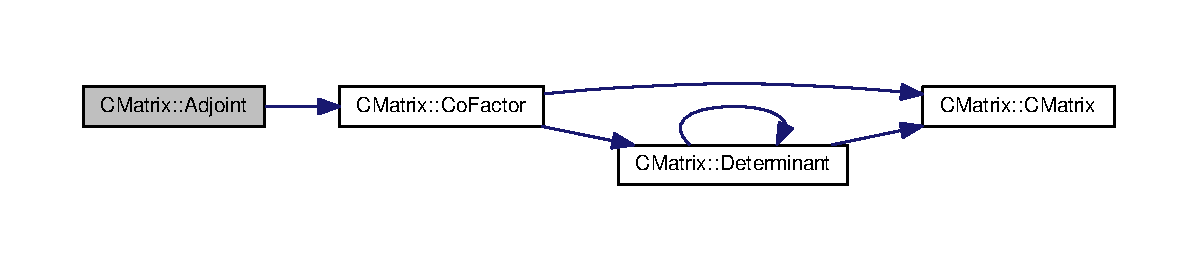
\includegraphics[width=350pt]{classCMatrix_a029eef7850029d78359ba09607cd8457_cgraph}
\end{center}
\end{figure}


\index{C\+Matrix@{C\+Matrix}!Co\+Factor@{Co\+Factor}}
\index{Co\+Factor@{Co\+Factor}!C\+Matrix@{C\+Matrix}}
\subsubsection[{\texorpdfstring{Co\+Factor()}{CoFactor()}}]{\setlength{\rightskip}{0pt plus 5cm}{\bf C\+Matrix} C\+Matrix\+::\+Co\+Factor (
\begin{DoxyParamCaption}
{}
\end{DoxyParamCaption}
)\hspace{0.3cm}{\ttfamily [inline]}}\hypertarget{classCMatrix_acc5e18f7dac42418762e92ebd8d10840}{}\label{classCMatrix_acc5e18f7dac42418762e92ebd8d10840}

\begin{DoxyCode}
258         \{
259             \hyperlink{classCMatrix}{CMatrix} cofactor(\textcolor{stringliteral}{"COF"}, \hyperlink{classCMatrix_ae23e5f8016ba06cfd1cce364a99f5037}{m\_rows}, \hyperlink{classCMatrix_a723f752208c055093012984eaddb62d3}{m\_cols});
260             \textcolor{keywordflow}{if} (\hyperlink{classCMatrix_ae23e5f8016ba06cfd1cce364a99f5037}{m\_rows} != \hyperlink{classCMatrix_a723f752208c055093012984eaddb62d3}{m\_cols})
261                 \textcolor{keywordflow}{return} cofactor;
262             \textcolor{keywordflow}{if} (\hyperlink{classCMatrix_ae23e5f8016ba06cfd1cce364a99f5037}{m\_rows} < 2)
263                 \textcolor{keywordflow}{return} cofactor;
264             \textcolor{keywordflow}{else} \textcolor{keywordflow}{if} (\hyperlink{classCMatrix_ae23e5f8016ba06cfd1cce364a99f5037}{m\_rows} == 2)
265             \{
266                 cofactor.m\_pData[0][0] = \hyperlink{classCMatrix_ab0f18d68cad9b6d750d05a96b60a759d}{m\_pData}[1][1];
267                 cofactor.m\_pData[0][1] = -\hyperlink{classCMatrix_ab0f18d68cad9b6d750d05a96b60a759d}{m\_pData}[1][0];
268                 cofactor.m\_pData[1][0] = -\hyperlink{classCMatrix_ab0f18d68cad9b6d750d05a96b60a759d}{m\_pData}[0][1];
269                 cofactor.m\_pData[1][1] = \hyperlink{classCMatrix_ab0f18d68cad9b6d750d05a96b60a759d}{m\_pData}[0][0];
270                 \textcolor{keywordflow}{return} cofactor;
271             \}
272             \textcolor{keywordflow}{else} \textcolor{keywordflow}{if} (\hyperlink{classCMatrix_ae23e5f8016ba06cfd1cce364a99f5037}{m\_rows} >= 3)
273             \{
274                 \textcolor{keywordtype}{int} DIM = \hyperlink{classCMatrix_ae23e5f8016ba06cfd1cce364a99f5037}{m\_rows};
275                 \hyperlink{classCMatrix}{CMatrix} ***temp = \textcolor{keyword}{new} \hyperlink{classCMatrix}{CMatrix}**[DIM];
276                 \textcolor{keywordflow}{for} (\textcolor{keywordtype}{int} i = 0; i < DIM; i++)
277                     temp[i] = \textcolor{keyword}{new} \hyperlink{classCMatrix}{CMatrix}*[DIM];
278                 \textcolor{keywordflow}{for} (\textcolor{keywordtype}{int} i = 0; i < DIM; i++)
279                     \textcolor{keywordflow}{for} (\textcolor{keywordtype}{int} j = 0; j < DIM; j++)
280                         temp[i][j] = \textcolor{keyword}{new} \hyperlink{classCMatrix_a720aa6a48296f4414ac7f9021bc420c4}{CMatrix}(\textcolor{stringliteral}{""}, DIM - 1, DIM - 1);
281                 \textcolor{keywordflow}{for} (\textcolor{keywordtype}{int} k1 = 0; k1 < DIM; k1++)
282                 \{
283                     \textcolor{keywordflow}{for} (\textcolor{keywordtype}{int} k2 = 0; k2 < DIM; k2++)
284                     \{
285                         \textcolor{keywordtype}{int} i1 = 0;
286                         \textcolor{keywordflow}{for} (\textcolor{keywordtype}{int} i = 0; i < DIM; i++)
287                         \{
288                             \textcolor{keywordtype}{int} j1 = 0;
289                             \textcolor{keywordflow}{for} (\textcolor{keywordtype}{int} j = 0; j < DIM; j++)
290                             \{
291                                 \textcolor{keywordflow}{if} (k1 == i || k2 == j)
292                                     \textcolor{keywordflow}{continue};
293                                 temp[k1][k2]->\hyperlink{classCMatrix_ab0f18d68cad9b6d750d05a96b60a759d}{m\_pData}[i1][j1++]
294                                         = this->\hyperlink{classCMatrix_ab0f18d68cad9b6d750d05a96b60a759d}{m\_pData}[i][j];
295                             \}
296                             \textcolor{keywordflow}{if} (k1 != i)
297                                 i1++;
298                         \}
299                     \}
300                 \}
301                 \textcolor{keywordtype}{bool} flagPositive = \textcolor{keyword}{true};
302                 \textcolor{keywordflow}{for} (\textcolor{keywordtype}{int} k1 = 0; k1 < DIM; k1++)
303                 \{
304                     flagPositive = ((k1 % 2) == 0);
305                     \textcolor{keywordflow}{for} (\textcolor{keywordtype}{int} k2 = 0; k2 < DIM; k2++)
306                     \{
307                         \textcolor{keywordflow}{if} (flagPositive == \textcolor{keyword}{true})
308                         \{
309                             cofactor.m\_pData[k1][k2]
310                                     = temp[k1][k2]->\hyperlink{classCMatrix_a865ff8f610be372e666fbf24d5b73a3a}{Determinant}();
311                             flagPositive = \textcolor{keyword}{false};
312                         \}
313                         \textcolor{keywordflow}{else}
314                         \{
315                             cofactor.m\_pData[k1][k2]
316                                     = -temp[k1][k2]->\hyperlink{classCMatrix_a865ff8f610be372e666fbf24d5b73a3a}{Determinant}();
317                             flagPositive = \textcolor{keyword}{true};
318                         \}
319                     \}
320                 \}
321                 \textcolor{keywordflow}{for} (\textcolor{keywordtype}{int} i = 0; i < DIM; i++)
322                     \textcolor{keywordflow}{for} (\textcolor{keywordtype}{int} j = 0; j < DIM; j++)
323                         \textcolor{keyword}{delete} temp[i][j];
324                 \textcolor{keywordflow}{for} (\textcolor{keywordtype}{int} i = 0; i < DIM; i++)
325                     \textcolor{keyword}{delete}[] temp[i];
326                 \textcolor{keyword}{delete}[] temp;
327             \}
328             \textcolor{keywordflow}{return} cofactor;
329         \}
\end{DoxyCode}


Here is the call graph for this function\+:
\nopagebreak
\begin{figure}[H]
\begin{center}
\leavevmode
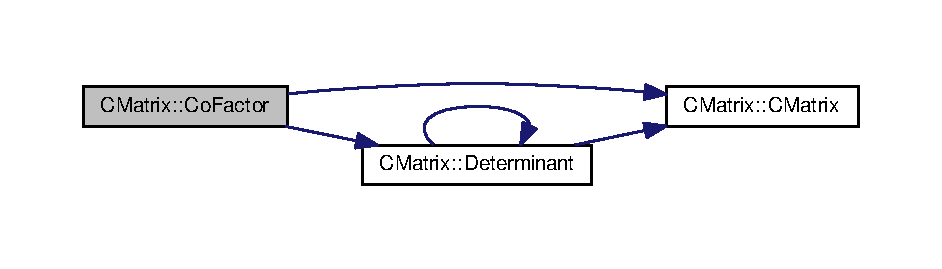
\includegraphics[width=350pt]{classCMatrix_acc5e18f7dac42418762e92ebd8d10840_cgraph}
\end{center}
\end{figure}


\index{C\+Matrix@{C\+Matrix}!Determinant@{Determinant}}
\index{Determinant@{Determinant}!C\+Matrix@{C\+Matrix}}
\subsubsection[{\texorpdfstring{Determinant()}{Determinant()}}]{\setlength{\rightskip}{0pt plus 5cm}double C\+Matrix\+::\+Determinant (
\begin{DoxyParamCaption}
{}
\end{DoxyParamCaption}
)\hspace{0.3cm}{\ttfamily [inline]}}\hypertarget{classCMatrix_a865ff8f610be372e666fbf24d5b73a3a}{}\label{classCMatrix_a865ff8f610be372e666fbf24d5b73a3a}

\begin{DoxyCode}
90         \{
91             \textcolor{keywordtype}{double} det = 0;
92             \textcolor{keywordtype}{double} **pd = \hyperlink{classCMatrix_ab0f18d68cad9b6d750d05a96b60a759d}{m\_pData};
93             \textcolor{keywordflow}{switch} (\hyperlink{classCMatrix_ae23e5f8016ba06cfd1cce364a99f5037}{m\_rows})
94             \{
95                 \textcolor{keywordflow}{case} 2:
96                 \{
97                     det = pd[0][0] * pd[1][1] - pd[0][1] * pd[1][0];
98                     \textcolor{keywordflow}{return} det;
99                 \}
100                     \textcolor{keywordflow}{break};
101                 \textcolor{keywordflow}{case} 3:
102                 \{
103                     \textcolor{comment}{/***}
104 \textcolor{comment}{                     a b c}
105 \textcolor{comment}{                     d e f}
106 \textcolor{comment}{                     g h i}
107 \textcolor{comment}{ }
108 \textcolor{comment}{                     a b c a b c}
109 \textcolor{comment}{                     d e f d e f}
110 \textcolor{comment}{                     g h i g h i}
111 \textcolor{comment}{ }
112 \textcolor{comment}{ }
113 \textcolor{comment}{                     // det (A) = aei + bfg + cdh - afh - bdi - ceg.}
114 \textcolor{comment}{                     ***/}
115                     \textcolor{keywordtype}{double} a = pd[0][0];
116                     \textcolor{keywordtype}{double} b = pd[0][1];
117                     \textcolor{keywordtype}{double} c = pd[0][2];
118                     \textcolor{keywordtype}{double} d = pd[1][0];
119                     \textcolor{keywordtype}{double} e = pd[1][1];
120                     \textcolor{keywordtype}{double} f = pd[1][2];
121                     \textcolor{keywordtype}{double} g = pd[2][0];
122                     \textcolor{keywordtype}{double} h = pd[2][1];
123                     \textcolor{keywordtype}{double} i = pd[2][2];
124                     \textcolor{keywordtype}{double} det = (a * e * i + b * f * g + c * d * h); \textcolor{comment}{// - a*f*h - b*d*i - c*e*g);}
125                     det = det - a * f * h;
126                     det = det - b * d * i;
127                     det = det - c * e * g;
128                     \textcolor{comment}{//std::cout << *this;}
129                     \textcolor{comment}{//std::cout << "deter: " << det << " \(\backslash\)n";}
130  
131                     \textcolor{keywordflow}{return} det;
132                 \}
133                     \textcolor{keywordflow}{break};
134                 \textcolor{keywordflow}{case} 4:
135                 \{
136                     \hyperlink{classCMatrix}{CMatrix} *temp[4];
137                     \textcolor{keywordflow}{for} (\textcolor{keywordtype}{int} i = 0; i < 4; i++)
138                         temp[i] = \textcolor{keyword}{new} \hyperlink{classCMatrix_a720aa6a48296f4414ac7f9021bc420c4}{CMatrix}(\textcolor{stringliteral}{""}, 3, 3);
139                     \textcolor{keywordflow}{for} (\textcolor{keywordtype}{int} k = 0; k < 4; k++)
140                     \{
141                         \textcolor{keywordflow}{for} (\textcolor{keywordtype}{int} i = 1; i < 4; i++)
142                         \{
143                             \textcolor{keywordtype}{int} j1 = 0;
144                             \textcolor{keywordflow}{for} (\textcolor{keywordtype}{int} j = 0; j < 4; j++)
145                             \{
146                                 \textcolor{keywordflow}{if} (k == j)
147                                     \textcolor{keywordflow}{continue};
148                                 temp[k]->\hyperlink{classCMatrix_ab0f18d68cad9b6d750d05a96b60a759d}{m\_pData}[i - 1][j1++]
149                                         = this->\hyperlink{classCMatrix_ab0f18d68cad9b6d750d05a96b60a759d}{m\_pData}[i][j];
150                             \}
151                         \}
152                     \}
153                     \textcolor{keywordtype}{double} det = this->\hyperlink{classCMatrix_ab0f18d68cad9b6d750d05a96b60a759d}{m\_pData}[0][0] * temp[0]->
      \hyperlink{classCMatrix_a865ff8f610be372e666fbf24d5b73a3a}{Determinant}()
154                             - this->\hyperlink{classCMatrix_ab0f18d68cad9b6d750d05a96b60a759d}{m\_pData}[0][1] * temp[1]->\hyperlink{classCMatrix_a865ff8f610be372e666fbf24d5b73a3a}{Determinant}()
155                             + this->\hyperlink{classCMatrix_ab0f18d68cad9b6d750d05a96b60a759d}{m\_pData}[0][2] * temp[2]->\hyperlink{classCMatrix_a865ff8f610be372e666fbf24d5b73a3a}{Determinant}()
156                             - this->\hyperlink{classCMatrix_ab0f18d68cad9b6d750d05a96b60a759d}{m\_pData}[0][3] * temp[3]->\hyperlink{classCMatrix_a865ff8f610be372e666fbf24d5b73a3a}{Determinant}();
157                     \textcolor{keywordflow}{return} det;
158                 \}
159                     \textcolor{keywordflow}{break};
160                 \textcolor{keywordflow}{case} 5:
161                 \{
162                     \hyperlink{classCMatrix}{CMatrix} *temp[5];
163                     \textcolor{keywordflow}{for} (\textcolor{keywordtype}{int} i = 0; i < 5; i++)
164                         temp[i] = \textcolor{keyword}{new} \hyperlink{classCMatrix_a720aa6a48296f4414ac7f9021bc420c4}{CMatrix}(\textcolor{stringliteral}{""}, 4, 4);
165                     \textcolor{keywordflow}{for} (\textcolor{keywordtype}{int} k = 0; k < 5; k++)
166                     \{
167                         \textcolor{keywordflow}{for} (\textcolor{keywordtype}{int} i = 1; i < 5; i++)
168                         \{
169                             \textcolor{keywordtype}{int} j1 = 0;
170                             \textcolor{keywordflow}{for} (\textcolor{keywordtype}{int} j = 0; j < 5; j++)
171                             \{
172                                 \textcolor{keywordflow}{if} (k == j)
173                                     \textcolor{keywordflow}{continue};
174                                 temp[k]->\hyperlink{classCMatrix_ab0f18d68cad9b6d750d05a96b60a759d}{m\_pData}[i - 1][j1++]
175                                         = this->\hyperlink{classCMatrix_ab0f18d68cad9b6d750d05a96b60a759d}{m\_pData}[i][j];
176                             \}
177                         \}
178                     \}
179                     \textcolor{keywordtype}{double} det = this->\hyperlink{classCMatrix_ab0f18d68cad9b6d750d05a96b60a759d}{m\_pData}[0][0] * temp[0]->
      \hyperlink{classCMatrix_a865ff8f610be372e666fbf24d5b73a3a}{Determinant}()
180                             - this->\hyperlink{classCMatrix_ab0f18d68cad9b6d750d05a96b60a759d}{m\_pData}[0][1] * temp[1]->\hyperlink{classCMatrix_a865ff8f610be372e666fbf24d5b73a3a}{Determinant}()
181                             + this->\hyperlink{classCMatrix_ab0f18d68cad9b6d750d05a96b60a759d}{m\_pData}[0][2] * temp[2]->\hyperlink{classCMatrix_a865ff8f610be372e666fbf24d5b73a3a}{Determinant}()
182                             - this->\hyperlink{classCMatrix_ab0f18d68cad9b6d750d05a96b60a759d}{m\_pData}[0][3] * temp[3]->\hyperlink{classCMatrix_a865ff8f610be372e666fbf24d5b73a3a}{Determinant}()
183                             + this->\hyperlink{classCMatrix_ab0f18d68cad9b6d750d05a96b60a759d}{m\_pData}[0][4] * temp[4]->\hyperlink{classCMatrix_a865ff8f610be372e666fbf24d5b73a3a}{Determinant}();
184                     \textcolor{keywordflow}{return} det;
185                 \}
186                 \textcolor{keywordflow}{case} 6:
187                 \textcolor{keywordflow}{case} 7:
188                 \textcolor{keywordflow}{case} 8:
189                 \textcolor{keywordflow}{case} 9:
190                 \textcolor{keywordflow}{case} 10:
191                 \textcolor{keywordflow}{case} 11:
192                 \textcolor{keywordflow}{case} 12:
193                 \textcolor{keywordflow}{default}:
194                 \{
195                     \textcolor{keywordtype}{int} DIM = \hyperlink{classCMatrix_ae23e5f8016ba06cfd1cce364a99f5037}{m\_rows};
196                     \hyperlink{classCMatrix}{CMatrix} **temp = \textcolor{keyword}{new} \hyperlink{classCMatrix}{CMatrix}*[DIM];
197                     \textcolor{keywordflow}{for} (\textcolor{keywordtype}{int} i = 0; i < DIM; i++)
198                         temp[i] = \textcolor{keyword}{new} \hyperlink{classCMatrix_a720aa6a48296f4414ac7f9021bc420c4}{CMatrix}(\textcolor{stringliteral}{""}, DIM - 1, DIM - 1);
199                     \textcolor{keywordflow}{for} (\textcolor{keywordtype}{int} k = 0; k < DIM; k++)
200                     \{
201                         \textcolor{keywordflow}{for} (\textcolor{keywordtype}{int} i = 1; i < DIM; i++)
202                         \{
203                             \textcolor{keywordtype}{int} j1 = 0;
204                             \textcolor{keywordflow}{for} (\textcolor{keywordtype}{int} j = 0; j < DIM; j++)
205                             \{
206                                 \textcolor{keywordflow}{if} (k == j)
207                                     \textcolor{keywordflow}{continue};
208                                 temp[k]->\hyperlink{classCMatrix_ab0f18d68cad9b6d750d05a96b60a759d}{m\_pData}[i - 1][j1++]
209                                         = this->\hyperlink{classCMatrix_ab0f18d68cad9b6d750d05a96b60a759d}{m\_pData}[i][j];
210                             \}
211                         \}
212                     \}
213                     \textcolor{keywordtype}{double} det = 0;
214                     \textcolor{keywordflow}{for} (\textcolor{keywordtype}{int} k = 0; k < DIM; k++)
215                     \{
216                         \textcolor{keywordflow}{if} ((k % 2) == 0)
217                             det = det + (this->\hyperlink{classCMatrix_ab0f18d68cad9b6d750d05a96b60a759d}{m\_pData}[0][k]
218                                     * temp[k]->\hyperlink{classCMatrix_a865ff8f610be372e666fbf24d5b73a3a}{Determinant}());
219                         \textcolor{keywordflow}{else}
220                             det = det - (this->\hyperlink{classCMatrix_ab0f18d68cad9b6d750d05a96b60a759d}{m\_pData}[0][k]
221                                     * temp[k]->\hyperlink{classCMatrix_a865ff8f610be372e666fbf24d5b73a3a}{Determinant}());
222                     \}
223                     \textcolor{keywordflow}{for} (\textcolor{keywordtype}{int} i = 0; i < DIM; i++)
224                         \textcolor{keyword}{delete} temp[i];
225                     \textcolor{keyword}{delete}[] temp;
226                     \textcolor{keywordflow}{return} det;
227                 \}
228                     \textcolor{keywordflow}{break};
229             \}
230         \}
\end{DoxyCode}


Here is the call graph for this function\+:
\nopagebreak
\begin{figure}[H]
\begin{center}
\leavevmode
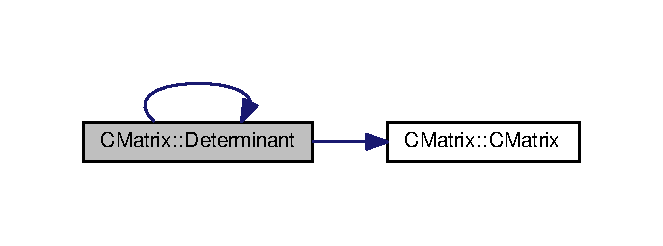
\includegraphics[width=318pt]{classCMatrix_a865ff8f610be372e666fbf24d5b73a3a_cgraph}
\end{center}
\end{figure}


\index{C\+Matrix@{C\+Matrix}!Fill\+Simulated\+Input@{Fill\+Simulated\+Input}}
\index{Fill\+Simulated\+Input@{Fill\+Simulated\+Input}!C\+Matrix@{C\+Matrix}}
\subsubsection[{\texorpdfstring{Fill\+Simulated\+Input()}{FillSimulatedInput()}}]{\setlength{\rightskip}{0pt plus 5cm}void C\+Matrix\+::\+Fill\+Simulated\+Input (
\begin{DoxyParamCaption}
{}
\end{DoxyParamCaption}
)\hspace{0.3cm}{\ttfamily [inline]}}\hypertarget{classCMatrix_afd8bcbf3b820b37223886632251e4d55}{}\label{classCMatrix_afd8bcbf3b820b37223886632251e4d55}

\begin{DoxyCode}
69         \{
70             \textcolor{keyword}{static} \textcolor{keywordtype}{int} factor1 = 1, factor2 = 2;
71             std::cout << \textcolor{stringliteral}{"\(\backslash\)n\(\backslash\)nEnter Input For Matrix : "} << \hyperlink{classCMatrix_aecd316cc4360014e817f7dc763aaa957}{m\_name} << \textcolor{stringliteral}{" Rows: "}
72                     << \hyperlink{classCMatrix_ae23e5f8016ba06cfd1cce364a99f5037}{m\_rows} << \textcolor{stringliteral}{" Cols: "} << \hyperlink{classCMatrix_a723f752208c055093012984eaddb62d3}{m\_cols} << \textcolor{stringliteral}{"\(\backslash\)n"};
73             \textcolor{keywordflow}{for} (\textcolor{keywordtype}{int} i = 0; i < \hyperlink{classCMatrix_ae23e5f8016ba06cfd1cce364a99f5037}{m\_rows}; i++)
74             \{
75                 \textcolor{keywordflow}{for} (\textcolor{keywordtype}{int} j = 0; j < \hyperlink{classCMatrix_a723f752208c055093012984eaddb62d3}{m\_cols}; j++)
76                 \{
77                     std::cout << \textcolor{stringliteral}{"Input For Row: "} << i + 1 << \textcolor{stringliteral}{" Col: "} << j
78                             + 1 << \textcolor{stringliteral}{" = "};
79                     \textcolor{keywordtype}{int} data = ((i + 1) * factor1) + (j + 1) * factor2;
80                     \hyperlink{classCMatrix_ab0f18d68cad9b6d750d05a96b60a759d}{m\_pData}[i][j] = data / 10.2;
81                     std::cout << \hyperlink{classCMatrix_ab0f18d68cad9b6d750d05a96b60a759d}{m\_pData}[i][j] << \textcolor{stringliteral}{"\(\backslash\)n"};
82                     factor1 += (rand() % 4);
83                     factor2 += (rand() % 3);
84                 \}
85                 std::cout << \textcolor{stringliteral}{"\(\backslash\)n"};
86             \}
87             std::cout << \textcolor{stringliteral}{"\(\backslash\)n"};
88         \}
\end{DoxyCode}
\index{C\+Matrix@{C\+Matrix}!Get\+Input@{Get\+Input}}
\index{Get\+Input@{Get\+Input}!C\+Matrix@{C\+Matrix}}
\subsubsection[{\texorpdfstring{Get\+Input()}{GetInput()}}]{\setlength{\rightskip}{0pt plus 5cm}void C\+Matrix\+::\+Get\+Input (
\begin{DoxyParamCaption}
{}
\end{DoxyParamCaption}
)\hspace{0.3cm}{\ttfamily [inline]}}\hypertarget{classCMatrix_af90c46bd02b2a57c58ffcff64d8dd3c6}{}\label{classCMatrix_af90c46bd02b2a57c58ffcff64d8dd3c6}

\begin{DoxyCode}
65         \{
66             std::cin >> *\textcolor{keyword}{this};
67         \}
\end{DoxyCode}
\index{C\+Matrix@{C\+Matrix}!Get\+Name@{Get\+Name}}
\index{Get\+Name@{Get\+Name}!C\+Matrix@{C\+Matrix}}
\subsubsection[{\texorpdfstring{Get\+Name() const }{GetName() const }}]{\setlength{\rightskip}{0pt plus 5cm}const char$\ast$ C\+Matrix\+::\+Get\+Name (
\begin{DoxyParamCaption}
{}
\end{DoxyParamCaption}
) const\hspace{0.3cm}{\ttfamily [inline]}}\hypertarget{classCMatrix_ae6df44c34368fbad7a5bfbda879af3ee}{}\label{classCMatrix_ae6df44c34368fbad7a5bfbda879af3ee}

\begin{DoxyCode}
61         \{
62             \textcolor{keywordflow}{return} \hyperlink{classCMatrix_aecd316cc4360014e817f7dc763aaa957}{m\_name};
63         \}
\end{DoxyCode}
\index{C\+Matrix@{C\+Matrix}!Inverse@{Inverse}}
\index{Inverse@{Inverse}!C\+Matrix@{C\+Matrix}}
\subsubsection[{\texorpdfstring{Inverse()}{Inverse()}}]{\setlength{\rightskip}{0pt plus 5cm}{\bf C\+Matrix} C\+Matrix\+::\+Inverse (
\begin{DoxyParamCaption}
{}
\end{DoxyParamCaption}
)\hspace{0.3cm}{\ttfamily [inline]}}\hypertarget{classCMatrix_abd58298df23c98b8675a81a70c6f140b}{}\label{classCMatrix_abd58298df23c98b8675a81a70c6f140b}

\begin{DoxyCode}
360         \{
361             \hyperlink{classCMatrix}{CMatrix} cofactor(\textcolor{stringliteral}{"COF"}, \hyperlink{classCMatrix_ae23e5f8016ba06cfd1cce364a99f5037}{m\_rows}, \hyperlink{classCMatrix_a723f752208c055093012984eaddb62d3}{m\_cols});
362             \hyperlink{classCMatrix}{CMatrix} inv(\textcolor{stringliteral}{"INV"}, \hyperlink{classCMatrix_ae23e5f8016ba06cfd1cce364a99f5037}{m\_rows}, \hyperlink{classCMatrix_a723f752208c055093012984eaddb62d3}{m\_cols});
363             \textcolor{keywordflow}{if} (\hyperlink{classCMatrix_ae23e5f8016ba06cfd1cce364a99f5037}{m\_rows} != \hyperlink{classCMatrix_a723f752208c055093012984eaddb62d3}{m\_cols})
364                 \textcolor{keywordflow}{return} inv;
365             \textcolor{comment}{// to find out Determinant}
366             \textcolor{keywordtype}{double} det = \hyperlink{classCMatrix_a865ff8f610be372e666fbf24d5b73a3a}{Determinant}();
367             cofactor = this->\hyperlink{classCMatrix_acc5e18f7dac42418762e92ebd8d10840}{CoFactor}();
368             \textcolor{comment}{// inv = transpose of cofactor / Determinant}
369             \textcolor{keywordflow}{for} (\textcolor{keywordtype}{int} i = 0; i < \hyperlink{classCMatrix_ae23e5f8016ba06cfd1cce364a99f5037}{m\_rows}; i++)
370             \{
371                 \textcolor{keywordflow}{for} (\textcolor{keywordtype}{int} j = 0; j < \hyperlink{classCMatrix_a723f752208c055093012984eaddb62d3}{m\_cols}; j++)
372                 \{
373                     inv.m\_pData[j][i] = cofactor.m\_pData[i][j] / det;
374                 \}
375             \}
376             \textcolor{keywordflow}{return} inv;
377         \}
\end{DoxyCode}


Here is the call graph for this function\+:
\nopagebreak
\begin{figure}[H]
\begin{center}
\leavevmode
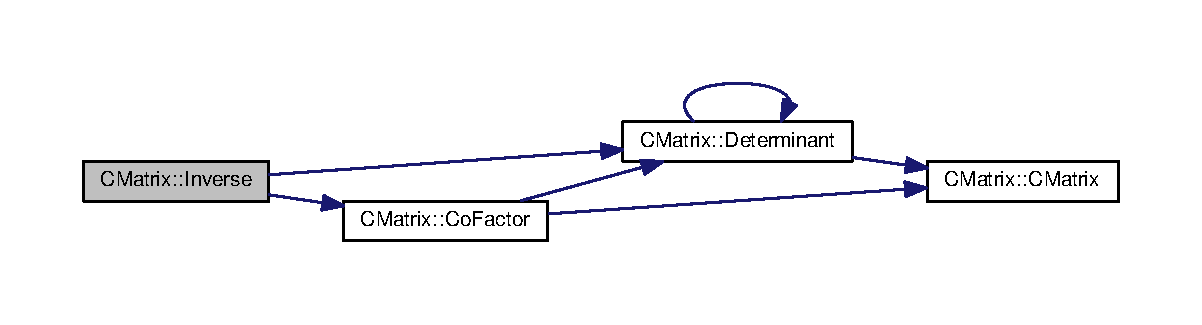
\includegraphics[width=350pt]{classCMatrix_abd58298df23c98b8675a81a70c6f140b_cgraph}
\end{center}
\end{figure}


\index{C\+Matrix@{C\+Matrix}!operator$\ast$@{operator$\ast$}}
\index{operator$\ast$@{operator$\ast$}!C\+Matrix@{C\+Matrix}}
\subsubsection[{\texorpdfstring{operator$\ast$(const C\+Matrix \&other)}{operator*(const CMatrix &other)}}]{\setlength{\rightskip}{0pt plus 5cm}{\bf C\+Matrix} C\+Matrix\+::operator$\ast$ (
\begin{DoxyParamCaption}
\item[{const {\bf C\+Matrix} \&}]{other}
\end{DoxyParamCaption}
)\hspace{0.3cm}{\ttfamily [inline]}}\hypertarget{classCMatrix_a665fdcc1fda1a9a23e6128f1ec31cc69}{}\label{classCMatrix_a665fdcc1fda1a9a23e6128f1ec31cc69}

\begin{DoxyCode}
417         \{
418             \textcolor{keywordflow}{if} (this->\hyperlink{classCMatrix_a723f752208c055093012984eaddb62d3}{m\_cols} != other.\hyperlink{classCMatrix_ae23e5f8016ba06cfd1cce364a99f5037}{m\_rows})
419             \{
420                 std::cout
421                         << \textcolor{stringliteral}{"Multiplication could not take place because number of columns of 1st Matrix and
       number of rows in 2nd Matrix are different"};
422                 \textcolor{keywordflow}{return} *\textcolor{keyword}{this};
423             \}
424             \hyperlink{classCMatrix}{CMatrix} result(\textcolor{stringliteral}{""}, this->\hyperlink{classCMatrix_ae23e5f8016ba06cfd1cce364a99f5037}{m\_rows}, other.\hyperlink{classCMatrix_a723f752208c055093012984eaddb62d3}{m\_cols});
425             \textcolor{keywordflow}{for} (\textcolor{keywordtype}{int} i = 0; i < this->\hyperlink{classCMatrix_ae23e5f8016ba06cfd1cce364a99f5037}{m\_rows}; i++)
426             \{
427                 \textcolor{keywordflow}{for} (\textcolor{keywordtype}{int} j = 0; j < other.\hyperlink{classCMatrix_a723f752208c055093012984eaddb62d3}{m\_cols}; j++)
428                 \{
429                     \textcolor{keywordflow}{for} (\textcolor{keywordtype}{int} k = 0; k < this->\hyperlink{classCMatrix_a723f752208c055093012984eaddb62d3}{m\_cols}; k++)
430                     \{
431                         result.m\_pData[i][j] += this->\hyperlink{classCMatrix_ab0f18d68cad9b6d750d05a96b60a759d}{m\_pData}[i][k]
432                                 * other.\hyperlink{classCMatrix_ab0f18d68cad9b6d750d05a96b60a759d}{m\_pData}[k][j];
433                     \}
434                 \}
435             \}
436             \textcolor{keywordflow}{return} result;
437         \}
\end{DoxyCode}
\index{C\+Matrix@{C\+Matrix}!operator+@{operator+}}
\index{operator+@{operator+}!C\+Matrix@{C\+Matrix}}
\subsubsection[{\texorpdfstring{operator+(const C\+Matrix \&other)}{operator+(const CMatrix &other)}}]{\setlength{\rightskip}{0pt plus 5cm}{\bf C\+Matrix} C\+Matrix\+::operator+ (
\begin{DoxyParamCaption}
\item[{const {\bf C\+Matrix} \&}]{other}
\end{DoxyParamCaption}
)\hspace{0.3cm}{\ttfamily [inline]}}\hypertarget{classCMatrix_a0fac0198450dcbcd402e1802dd6b8008}{}\label{classCMatrix_a0fac0198450dcbcd402e1802dd6b8008}

\begin{DoxyCode}
379         \{
380             \textcolor{keywordflow}{if} (this->\hyperlink{classCMatrix_ae23e5f8016ba06cfd1cce364a99f5037}{m\_rows} != other.\hyperlink{classCMatrix_ae23e5f8016ba06cfd1cce364a99f5037}{m\_rows} || this->m\_cols != other.
      \hyperlink{classCMatrix_a723f752208c055093012984eaddb62d3}{m\_cols})
381             \{
382                 std::cout
383                         << \textcolor{stringliteral}{"Addition could not take place because number of rows and columns are different
       between the two matrices"};
384                 \textcolor{keywordflow}{return} *\textcolor{keyword}{this};
385             \}
386             \hyperlink{classCMatrix}{CMatrix} result(\textcolor{stringliteral}{""}, \hyperlink{classCMatrix_ae23e5f8016ba06cfd1cce364a99f5037}{m\_rows}, \hyperlink{classCMatrix_a723f752208c055093012984eaddb62d3}{m\_cols});
387             \textcolor{keywordflow}{for} (\textcolor{keywordtype}{int} i = 0; i < \hyperlink{classCMatrix_ae23e5f8016ba06cfd1cce364a99f5037}{m\_rows}; i++)
388             \{
389                 \textcolor{keywordflow}{for} (\textcolor{keywordtype}{int} j = 0; j < \hyperlink{classCMatrix_a723f752208c055093012984eaddb62d3}{m\_cols}; j++)
390                 \{
391                     result.m\_pData[i][j] = this->\hyperlink{classCMatrix_ab0f18d68cad9b6d750d05a96b60a759d}{m\_pData}[i][j]
392                             + other.\hyperlink{classCMatrix_ab0f18d68cad9b6d750d05a96b60a759d}{m\_pData}[i][j];
393                 \}
394             \}
395             \textcolor{keywordflow}{return} result;
396         \}
\end{DoxyCode}
\index{C\+Matrix@{C\+Matrix}!operator-\/@{operator-\/}}
\index{operator-\/@{operator-\/}!C\+Matrix@{C\+Matrix}}
\subsubsection[{\texorpdfstring{operator-\/(const C\+Matrix \&other)}{operator-(const CMatrix &other)}}]{\setlength{\rightskip}{0pt plus 5cm}{\bf C\+Matrix} C\+Matrix\+::operator-\/ (
\begin{DoxyParamCaption}
\item[{const {\bf C\+Matrix} \&}]{other}
\end{DoxyParamCaption}
)\hspace{0.3cm}{\ttfamily [inline]}}\hypertarget{classCMatrix_a26d893cfb384a7c23f5c2c959fe74293}{}\label{classCMatrix_a26d893cfb384a7c23f5c2c959fe74293}

\begin{DoxyCode}
398         \{
399             \textcolor{keywordflow}{if} (this->\hyperlink{classCMatrix_ae23e5f8016ba06cfd1cce364a99f5037}{m\_rows} != other.\hyperlink{classCMatrix_ae23e5f8016ba06cfd1cce364a99f5037}{m\_rows} || this->m\_cols != other.
      \hyperlink{classCMatrix_a723f752208c055093012984eaddb62d3}{m\_cols})
400             \{
401                 std::cout
402                         << \textcolor{stringliteral}{"Subtraction could not take place because number of rows and columns are
       different between the two matrices"};
403                 \textcolor{keywordflow}{return} *\textcolor{keyword}{this};
404             \}
405             \hyperlink{classCMatrix}{CMatrix} result(\textcolor{stringliteral}{""}, \hyperlink{classCMatrix_ae23e5f8016ba06cfd1cce364a99f5037}{m\_rows}, \hyperlink{classCMatrix_a723f752208c055093012984eaddb62d3}{m\_cols});
406             \textcolor{keywordflow}{for} (\textcolor{keywordtype}{int} i = 0; i < \hyperlink{classCMatrix_ae23e5f8016ba06cfd1cce364a99f5037}{m\_rows}; i++)
407             \{
408                 \textcolor{keywordflow}{for} (\textcolor{keywordtype}{int} j = 0; j < \hyperlink{classCMatrix_a723f752208c055093012984eaddb62d3}{m\_cols}; j++)
409                 \{
410                     result.m\_pData[i][j] = this->\hyperlink{classCMatrix_ab0f18d68cad9b6d750d05a96b60a759d}{m\_pData}[i][j]
411                             - other.\hyperlink{classCMatrix_ab0f18d68cad9b6d750d05a96b60a759d}{m\_pData}[i][j];
412                 \}
413             \}
414             \textcolor{keywordflow}{return} result;
415         \}
\end{DoxyCode}
\index{C\+Matrix@{C\+Matrix}!operator=@{operator=}}
\index{operator=@{operator=}!C\+Matrix@{C\+Matrix}}
\subsubsection[{\texorpdfstring{operator=(const C\+Matrix \&other)}{operator=(const CMatrix &other)}}]{\setlength{\rightskip}{0pt plus 5cm}{\bf C\+Matrix}\& C\+Matrix\+::operator= (
\begin{DoxyParamCaption}
\item[{const {\bf C\+Matrix} \&}]{other}
\end{DoxyParamCaption}
)\hspace{0.3cm}{\ttfamily [inline]}}\hypertarget{classCMatrix_a939d852e81803eddaac29d96d0a1ef84}{}\label{classCMatrix_a939d852e81803eddaac29d96d0a1ef84}

\begin{DoxyCode}
232         \{
233             \textcolor{keywordflow}{if} (this->\hyperlink{classCMatrix_ae23e5f8016ba06cfd1cce364a99f5037}{m\_rows} != other.\hyperlink{classCMatrix_ae23e5f8016ba06cfd1cce364a99f5037}{m\_rows} || this->m\_cols != other.
      \hyperlink{classCMatrix_a723f752208c055093012984eaddb62d3}{m\_cols})
234             \{
235                 std::cout
236                         << \textcolor{stringliteral}{"WARNING: Assignment is taking place with by changing the number of rows and
       columns of the matrix"};
237             \}
238             \textcolor{keywordflow}{for} (\textcolor{keywordtype}{int} i = 0; i < \hyperlink{classCMatrix_ae23e5f8016ba06cfd1cce364a99f5037}{m\_rows}; i++)
239                 \textcolor{keyword}{delete}[] \hyperlink{classCMatrix_ab0f18d68cad9b6d750d05a96b60a759d}{m\_pData}[i];
240             \textcolor{keyword}{delete}[] \hyperlink{classCMatrix_ab0f18d68cad9b6d750d05a96b60a759d}{m\_pData};
241             m\_rows = \hyperlink{classCMatrix_a723f752208c055093012984eaddb62d3}{m\_cols} = 0;
242             strcpy(\hyperlink{classCMatrix_aecd316cc4360014e817f7dc763aaa957}{m\_name}, other.\hyperlink{classCMatrix_aecd316cc4360014e817f7dc763aaa957}{m\_name});
243             m\_rows = other.\hyperlink{classCMatrix_ae23e5f8016ba06cfd1cce364a99f5037}{m\_rows};
244             \hyperlink{classCMatrix_a723f752208c055093012984eaddb62d3}{m\_cols} = other.\hyperlink{classCMatrix_a723f752208c055093012984eaddb62d3}{m\_cols};
245             \hyperlink{classCMatrix_ab0f18d68cad9b6d750d05a96b60a759d}{m\_pData} = \textcolor{keyword}{new} \textcolor{keywordtype}{double}*[\hyperlink{classCMatrix_ae23e5f8016ba06cfd1cce364a99f5037}{m\_rows}];
246             \textcolor{keywordflow}{for} (\textcolor{keywordtype}{int} i = 0; i < \hyperlink{classCMatrix_ae23e5f8016ba06cfd1cce364a99f5037}{m\_rows}; i++)
247                 \hyperlink{classCMatrix_ab0f18d68cad9b6d750d05a96b60a759d}{m\_pData}[i] = \textcolor{keyword}{new} \textcolor{keywordtype}{double}[\hyperlink{classCMatrix_a723f752208c055093012984eaddb62d3}{m\_cols}];
248             \textcolor{keywordflow}{for} (\textcolor{keywordtype}{int} i = 0; i < \hyperlink{classCMatrix_ae23e5f8016ba06cfd1cce364a99f5037}{m\_rows}; i++)
249             \{
250                 \textcolor{keywordflow}{for} (\textcolor{keywordtype}{int} j = 0; j < \hyperlink{classCMatrix_a723f752208c055093012984eaddb62d3}{m\_cols}; j++)
251                 \{
252                     \hyperlink{classCMatrix_ab0f18d68cad9b6d750d05a96b60a759d}{m\_pData}[i][j] = other.\hyperlink{classCMatrix_ab0f18d68cad9b6d750d05a96b60a759d}{m\_pData}[i][j];
253                 \}
254             \}
255             \textcolor{keywordflow}{return} *\textcolor{keyword}{this};
256         \}
\end{DoxyCode}
\index{C\+Matrix@{C\+Matrix}!operator==@{operator==}}
\index{operator==@{operator==}!C\+Matrix@{C\+Matrix}}
\subsubsection[{\texorpdfstring{operator==(const C\+Matrix \&other)}{operator==(const CMatrix &other)}}]{\setlength{\rightskip}{0pt plus 5cm}bool C\+Matrix\+::operator== (
\begin{DoxyParamCaption}
\item[{const {\bf C\+Matrix} \&}]{other}
\end{DoxyParamCaption}
)\hspace{0.3cm}{\ttfamily [inline]}}\hypertarget{classCMatrix_a2f26b64fa654512fe2a4e954f18e1f1c}{}\label{classCMatrix_a2f26b64fa654512fe2a4e954f18e1f1c}

\begin{DoxyCode}
439         \{
440             \textcolor{keywordflow}{if} (this->\hyperlink{classCMatrix_ae23e5f8016ba06cfd1cce364a99f5037}{m\_rows} != other.\hyperlink{classCMatrix_ae23e5f8016ba06cfd1cce364a99f5037}{m\_rows} || this->m\_cols != other.
      \hyperlink{classCMatrix_a723f752208c055093012984eaddb62d3}{m\_cols})
441             \{
442                 std::cout
443                         << \textcolor{stringliteral}{"Comparision could not take place because number of rows and columns are
       different between the two matrices"};
444                 \textcolor{keywordflow}{return} \textcolor{keyword}{false};
445             \}
446             \hyperlink{classCMatrix}{CMatrix} result(\textcolor{stringliteral}{""}, \hyperlink{classCMatrix_ae23e5f8016ba06cfd1cce364a99f5037}{m\_rows}, \hyperlink{classCMatrix_a723f752208c055093012984eaddb62d3}{m\_cols});
447             \textcolor{keywordtype}{bool} bEqual = \textcolor{keyword}{true};
448             \textcolor{keywordflow}{for} (\textcolor{keywordtype}{int} i = 0; i < \hyperlink{classCMatrix_ae23e5f8016ba06cfd1cce364a99f5037}{m\_rows}; i++)
449             \{
450                 \textcolor{keywordflow}{for} (\textcolor{keywordtype}{int} j = 0; j < \hyperlink{classCMatrix_a723f752208c055093012984eaddb62d3}{m\_cols}; j++)
451                 \{
452                     \textcolor{keywordflow}{if} (this->\hyperlink{classCMatrix_ab0f18d68cad9b6d750d05a96b60a759d}{m\_pData}[i][j] != other.\hyperlink{classCMatrix_ab0f18d68cad9b6d750d05a96b60a759d}{m\_pData}[i][j])
453                         bEqual = \textcolor{keyword}{false};
454                 \}
455             \}
456             \textcolor{keywordflow}{return} bEqual;
457         \}
\end{DoxyCode}
\index{C\+Matrix@{C\+Matrix}!Set\+Name@{Set\+Name}}
\index{Set\+Name@{Set\+Name}!C\+Matrix@{C\+Matrix}}
\subsubsection[{\texorpdfstring{Set\+Name(const char $\ast$name)}{SetName(const char *name)}}]{\setlength{\rightskip}{0pt plus 5cm}void C\+Matrix\+::\+Set\+Name (
\begin{DoxyParamCaption}
\item[{const char $\ast$}]{name}
\end{DoxyParamCaption}
)\hspace{0.3cm}{\ttfamily [inline]}}\hypertarget{classCMatrix_a7878287aa7b5a1404980ff08d3cfeb16}{}\label{classCMatrix_a7878287aa7b5a1404980ff08d3cfeb16}

\begin{DoxyCode}
57         \{
58             strcpy(\hyperlink{classCMatrix_aecd316cc4360014e817f7dc763aaa957}{m\_name}, name);
59         \}
\end{DoxyCode}
\index{C\+Matrix@{C\+Matrix}!Transpose@{Transpose}}
\index{Transpose@{Transpose}!C\+Matrix@{C\+Matrix}}
\subsubsection[{\texorpdfstring{Transpose()}{Transpose()}}]{\setlength{\rightskip}{0pt plus 5cm}{\bf C\+Matrix} C\+Matrix\+::\+Transpose (
\begin{DoxyParamCaption}
{}
\end{DoxyParamCaption}
)\hspace{0.3cm}{\ttfamily [inline]}}\hypertarget{classCMatrix_ab8e853a7df8e23889ab233523324ff29}{}\label{classCMatrix_ab8e853a7df8e23889ab233523324ff29}

\begin{DoxyCode}
348         \{
349             \hyperlink{classCMatrix}{CMatrix} trans(\textcolor{stringliteral}{"TR"}, \hyperlink{classCMatrix_a723f752208c055093012984eaddb62d3}{m\_cols}, \hyperlink{classCMatrix_ae23e5f8016ba06cfd1cce364a99f5037}{m\_rows});
350             \textcolor{keywordflow}{for} (\textcolor{keywordtype}{int} i = 0; i < \hyperlink{classCMatrix_ae23e5f8016ba06cfd1cce364a99f5037}{m\_rows}; i++)
351             \{
352                 \textcolor{keywordflow}{for} (\textcolor{keywordtype}{int} j = 0; j < \hyperlink{classCMatrix_a723f752208c055093012984eaddb62d3}{m\_cols}; j++)
353                 \{
354                     trans.m\_pData[j][i] = \hyperlink{classCMatrix_ab0f18d68cad9b6d750d05a96b60a759d}{m\_pData}[i][j];
355                 \}
356             \}
357             \textcolor{keywordflow}{return} trans;
358         \}
\end{DoxyCode}


\subsection{Friends And Related Function Documentation}
\index{C\+Matrix@{C\+Matrix}!operator$<$$<$@{operator$<$$<$}}
\index{operator$<$$<$@{operator$<$$<$}!C\+Matrix@{C\+Matrix}}
\subsubsection[{\texorpdfstring{operator$<$$<$}{operator<<}}]{\setlength{\rightskip}{0pt plus 5cm}std\+::ostream\& operator$<$$<$ (
\begin{DoxyParamCaption}
\item[{std\+::ostream \&}]{os, }
\item[{const {\bf C\+Matrix} \&}]{m}
\end{DoxyParamCaption}
)\hspace{0.3cm}{\ttfamily [friend]}}\hypertarget{classCMatrix_a62d7be0784c5982bf356f96493281902}{}\label{classCMatrix_a62d7be0784c5982bf356f96493281902}

\begin{DoxyCode}
479 \{
480     os << \textcolor{stringliteral}{"\(\backslash\)n\(\backslash\)nMatrix : "} << m.\hyperlink{classCMatrix_aecd316cc4360014e817f7dc763aaa957}{m\_name} << \textcolor{stringliteral}{" Rows: "} << m.\hyperlink{classCMatrix_ae23e5f8016ba06cfd1cce364a99f5037}{m\_rows} << \textcolor{stringliteral}{" Cols: "}
481             << m.\hyperlink{classCMatrix_a723f752208c055093012984eaddb62d3}{m\_cols} << \textcolor{stringliteral}{"\(\backslash\)n\(\backslash\)n"};
482     \textcolor{keywordflow}{for} (\textcolor{keywordtype}{int} i = 0; i < m.\hyperlink{classCMatrix_ae23e5f8016ba06cfd1cce364a99f5037}{m\_rows}; i++)
483     \{
484         os << \textcolor{stringliteral}{" | "};
485         \textcolor{keywordflow}{for} (\textcolor{keywordtype}{int} j = 0; j < m.\hyperlink{classCMatrix_a723f752208c055093012984eaddb62d3}{m\_cols}; j++)
486         \{
487             \textcolor{keywordtype}{char} buf[32];
488             \textcolor{keywordtype}{double} data = m.\hyperlink{classCMatrix_ab0f18d68cad9b6d750d05a96b60a759d}{m\_pData}[i][j];
489             \textcolor{keywordflow}{if} (m.\hyperlink{classCMatrix_ab0f18d68cad9b6d750d05a96b60a759d}{m\_pData}[i][j] > -0.00001 && m.\hyperlink{classCMatrix_ab0f18d68cad9b6d750d05a96b60a759d}{m\_pData}[i][j] < 0.00001)
490                 data = 0;
491             sprintf(buf, \textcolor{stringliteral}{"%10.2lf "}, data);
492             os << buf;
493         \}
494         os << \textcolor{stringliteral}{"|\(\backslash\)n"};
495     \}
496     os << \textcolor{stringliteral}{"\(\backslash\)n\(\backslash\)n"};
497     \textcolor{keywordflow}{return} os;
498 \}
\end{DoxyCode}
\index{C\+Matrix@{C\+Matrix}!operator$>$$>$@{operator$>$$>$}}
\index{operator$>$$>$@{operator$>$$>$}!C\+Matrix@{C\+Matrix}}
\subsubsection[{\texorpdfstring{operator$>$$>$}{operator>>}}]{\setlength{\rightskip}{0pt plus 5cm}std\+::istream\& operator$>$$>$ (
\begin{DoxyParamCaption}
\item[{std\+::istream \&}]{is, }
\item[{{\bf C\+Matrix} \&}]{m}
\end{DoxyParamCaption}
)\hspace{0.3cm}{\ttfamily [friend]}}\hypertarget{classCMatrix_a775d8b5122da5b9fdea41520953a4237}{}\label{classCMatrix_a775d8b5122da5b9fdea41520953a4237}

\begin{DoxyCode}
462 \{
463     std::cout << \textcolor{stringliteral}{"\(\backslash\)n\(\backslash\)nEnter Input For Matrix : "} << m.\hyperlink{classCMatrix_aecd316cc4360014e817f7dc763aaa957}{m\_name} << \textcolor{stringliteral}{" Rows: "}
464             << m.\hyperlink{classCMatrix_ae23e5f8016ba06cfd1cce364a99f5037}{m\_rows} << \textcolor{stringliteral}{" Cols: "} << m.\hyperlink{classCMatrix_a723f752208c055093012984eaddb62d3}{m\_cols} << \textcolor{stringliteral}{"\(\backslash\)n"};
465     \textcolor{keywordflow}{for} (\textcolor{keywordtype}{int} i = 0; i < m.\hyperlink{classCMatrix_ae23e5f8016ba06cfd1cce364a99f5037}{m\_rows}; i++)
466     \{
467         \textcolor{keywordflow}{for} (\textcolor{keywordtype}{int} j = 0; j < m.\hyperlink{classCMatrix_a723f752208c055093012984eaddb62d3}{m\_cols}; j++)
468         \{
469             std::cout << \textcolor{stringliteral}{"Input For Row: "} << i + 1 << \textcolor{stringliteral}{" Col: "} << j + 1
470                     << \textcolor{stringliteral}{" = "};
471             is >> m.\hyperlink{classCMatrix_ab0f18d68cad9b6d750d05a96b60a759d}{m\_pData}[i][j];
472         \}
473         std::cout << \textcolor{stringliteral}{"\(\backslash\)n"};
474     \}
475     std::cout << \textcolor{stringliteral}{"\(\backslash\)n"};
476     \textcolor{keywordflow}{return} is;
477 \}
\end{DoxyCode}


\subsection{Member Data Documentation}
\index{C\+Matrix@{C\+Matrix}!m\+\_\+cols@{m\+\_\+cols}}
\index{m\+\_\+cols@{m\+\_\+cols}!C\+Matrix@{C\+Matrix}}
\subsubsection[{\texorpdfstring{m\+\_\+cols}{m_cols}}]{\setlength{\rightskip}{0pt plus 5cm}int C\+Matrix\+::m\+\_\+cols\hspace{0.3cm}{\ttfamily [private]}}\hypertarget{classCMatrix_a723f752208c055093012984eaddb62d3}{}\label{classCMatrix_a723f752208c055093012984eaddb62d3}
\index{C\+Matrix@{C\+Matrix}!m\+\_\+name@{m\+\_\+name}}
\index{m\+\_\+name@{m\+\_\+name}!C\+Matrix@{C\+Matrix}}
\subsubsection[{\texorpdfstring{m\+\_\+name}{m_name}}]{\setlength{\rightskip}{0pt plus 5cm}char C\+Matrix\+::m\+\_\+name\mbox{[}128\mbox{]}\hspace{0.3cm}{\ttfamily [private]}}\hypertarget{classCMatrix_aecd316cc4360014e817f7dc763aaa957}{}\label{classCMatrix_aecd316cc4360014e817f7dc763aaa957}
\index{C\+Matrix@{C\+Matrix}!m\+\_\+p\+Data@{m\+\_\+p\+Data}}
\index{m\+\_\+p\+Data@{m\+\_\+p\+Data}!C\+Matrix@{C\+Matrix}}
\subsubsection[{\texorpdfstring{m\+\_\+p\+Data}{m_pData}}]{\setlength{\rightskip}{0pt plus 5cm}double$\ast$$\ast$ C\+Matrix\+::m\+\_\+p\+Data}\hypertarget{classCMatrix_ab0f18d68cad9b6d750d05a96b60a759d}{}\label{classCMatrix_ab0f18d68cad9b6d750d05a96b60a759d}
\index{C\+Matrix@{C\+Matrix}!m\+\_\+rows@{m\+\_\+rows}}
\index{m\+\_\+rows@{m\+\_\+rows}!C\+Matrix@{C\+Matrix}}
\subsubsection[{\texorpdfstring{m\+\_\+rows}{m_rows}}]{\setlength{\rightskip}{0pt plus 5cm}int C\+Matrix\+::m\+\_\+rows\hspace{0.3cm}{\ttfamily [private]}}\hypertarget{classCMatrix_ae23e5f8016ba06cfd1cce364a99f5037}{}\label{classCMatrix_ae23e5f8016ba06cfd1cce364a99f5037}


The documentation for this class was generated from the following file\+:\begin{DoxyCompactItemize}
\item 
\hyperlink{LinearEquation_8cpp}{Linear\+Equation.\+cpp}\end{DoxyCompactItemize}

\chapter{File Documentation}
\hypertarget{InverseMatrix_8cpp}{}\section{Inverse\+Matrix.\+cpp File Reference}
\label{InverseMatrix_8cpp}\index{Inverse\+Matrix.\+cpp@{Inverse\+Matrix.\+cpp}}
{\ttfamily \#include $<$stdio.\+h$>$}\\*
{\ttfamily \#include $<$iostream$>$}\\*
{\ttfamily \#include $<$tchar.\+h$>$}\\*
{\ttfamily \#include $<$math.\+h$>$}\\*
{\ttfamily \#include $<$stdlib.\+h$>$}\\*
Include dependency graph for Inverse\+Matrix.\+cpp\+:
\nopagebreak
\begin{figure}[H]
\begin{center}
\leavevmode
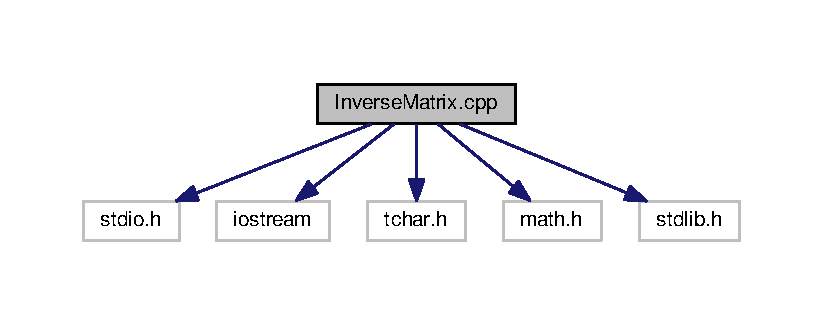
\includegraphics[width=350pt]{InverseMatrix_8cpp__incl}
\end{center}
\end{figure}
\subsection*{Classes}
\begin{DoxyCompactItemize}
\item 
class \hyperlink{classCMatrix}{C\+Matrix}
\end{DoxyCompactItemize}
\subsection*{Macros}
\begin{DoxyCompactItemize}
\item 
\#define \hyperlink{InverseMatrix_8cpp_a5b62c41f0c74994ce6ad7e0bed98cc51}{M\+A\+T\+R\+I\+X\+\_\+H}
\end{DoxyCompactItemize}
\subsection*{Functions}
\begin{DoxyCompactItemize}
\item 
std\+::istream \& \hyperlink{InverseMatrix_8cpp_a775d8b5122da5b9fdea41520953a4237}{operator$>$$>$} (std\+::istream \&is, \hyperlink{classCMatrix}{C\+Matrix} \&m)
\item 
std\+::ostream \& \hyperlink{InverseMatrix_8cpp_a62d7be0784c5982bf356f96493281902}{operator$<$$<$} (std\+::ostream \&os, const \hyperlink{classCMatrix}{C\+Matrix} \&m)
\item 
int \hyperlink{InverseMatrix_8cpp_ae66f6b31b5ad750f1fe042a706a4e3d4}{main} ()
\end{DoxyCompactItemize}


\subsection{Macro Definition Documentation}
\index{Inverse\+Matrix.\+cpp@{Inverse\+Matrix.\+cpp}!M\+A\+T\+R\+I\+X\+\_\+H@{M\+A\+T\+R\+I\+X\+\_\+H}}
\index{M\+A\+T\+R\+I\+X\+\_\+H@{M\+A\+T\+R\+I\+X\+\_\+H}!Inverse\+Matrix.\+cpp@{Inverse\+Matrix.\+cpp}}
\subsubsection[{\texorpdfstring{M\+A\+T\+R\+I\+X\+\_\+H}{MATRIX_H}}]{\setlength{\rightskip}{0pt plus 5cm}\#define M\+A\+T\+R\+I\+X\+\_\+H}\hypertarget{InverseMatrix_8cpp_a5b62c41f0c74994ce6ad7e0bed98cc51}{}\label{InverseMatrix_8cpp_a5b62c41f0c74994ce6ad7e0bed98cc51}


\subsection{Function Documentation}
\index{Inverse\+Matrix.\+cpp@{Inverse\+Matrix.\+cpp}!main@{main}}
\index{main@{main}!Inverse\+Matrix.\+cpp@{Inverse\+Matrix.\+cpp}}
\subsubsection[{\texorpdfstring{main()}{main()}}]{\setlength{\rightskip}{0pt plus 5cm}int main (
\begin{DoxyParamCaption}
{}
\end{DoxyParamCaption}
)}\hypertarget{InverseMatrix_8cpp_ae66f6b31b5ad750f1fe042a706a4e3d4}{}\label{InverseMatrix_8cpp_ae66f6b31b5ad750f1fe042a706a4e3d4}

\begin{DoxyCode}
497 \{
498     \hyperlink{classCMatrix}{CMatrix} a(\textcolor{stringliteral}{"A"}, 5, 5);
499     \textcolor{comment}{//std::cin >> a;}
500     a.FillSimulatedInput();
501     \hyperlink{classCMatrix}{CMatrix} aadj = a.\hyperlink{classCMatrix_abd58298df23c98b8675a81a70c6f140b}{Inverse}();
502     std::cout << a;
503     std::cout << aadj;
504     \hyperlink{classCMatrix}{CMatrix} unit = (a * aadj);
505     unit.\hyperlink{classCMatrix_a7878287aa7b5a1404980ff08d3cfeb16}{SetName}(\textcolor{stringliteral}{"A * A-Inv"});
506     std::cout << unit;
507 \}\end{DoxyCode}


Here is the call graph for this function\+:
\nopagebreak
\begin{figure}[H]
\begin{center}
\leavevmode
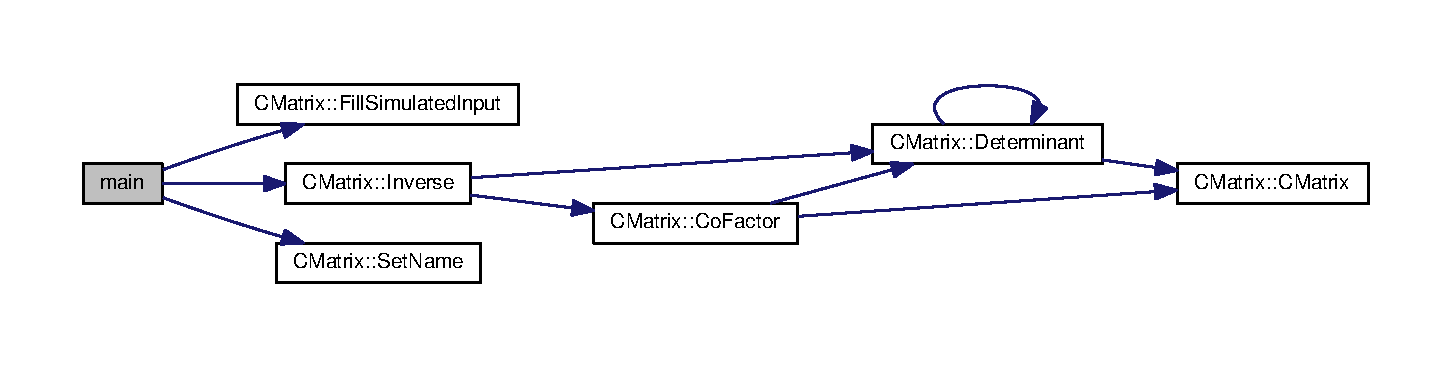
\includegraphics[width=350pt]{InverseMatrix_8cpp_ae66f6b31b5ad750f1fe042a706a4e3d4_cgraph}
\end{center}
\end{figure}


\index{Inverse\+Matrix.\+cpp@{Inverse\+Matrix.\+cpp}!operator$<$$<$@{operator$<$$<$}}
\index{operator$<$$<$@{operator$<$$<$}!Inverse\+Matrix.\+cpp@{Inverse\+Matrix.\+cpp}}
\subsubsection[{\texorpdfstring{operator$<$$<$(std\+::ostream \&os, const C\+Matrix \&m)}{operator<<(std::ostream &os, const CMatrix &m)}}]{\setlength{\rightskip}{0pt plus 5cm}std\+::ostream\& operator$<$$<$ (
\begin{DoxyParamCaption}
\item[{std\+::ostream \&}]{os, }
\item[{const {\bf C\+Matrix} \&}]{m}
\end{DoxyParamCaption}
)}\hypertarget{InverseMatrix_8cpp_a62d7be0784c5982bf356f96493281902}{}\label{InverseMatrix_8cpp_a62d7be0784c5982bf356f96493281902}

\begin{DoxyCode}
474 \{
475  
476     os << \textcolor{stringliteral}{"\(\backslash\)n\(\backslash\)nMatrix : "} << m.\hyperlink{classCMatrix_aecd316cc4360014e817f7dc763aaa957}{m\_name} << \textcolor{stringliteral}{" Rows: "} << m.\hyperlink{classCMatrix_ae23e5f8016ba06cfd1cce364a99f5037}{m\_rows} << \textcolor{stringliteral}{" Cols: "}
477             << m.\hyperlink{classCMatrix_a723f752208c055093012984eaddb62d3}{m\_cols} << \textcolor{stringliteral}{"\(\backslash\)n\(\backslash\)n"};
478     \textcolor{keywordflow}{for} (\textcolor{keywordtype}{int} i = 0; i < m.\hyperlink{classCMatrix_ae23e5f8016ba06cfd1cce364a99f5037}{m\_rows}; i++)
479     \{
480         os << \textcolor{stringliteral}{" | "};
481         \textcolor{keywordflow}{for} (\textcolor{keywordtype}{int} j = 0; j < m.\hyperlink{classCMatrix_a723f752208c055093012984eaddb62d3}{m\_cols}; j++)
482         \{
483             \textcolor{keywordtype}{char} buf[32];
484             \textcolor{keywordtype}{double} data = m.\hyperlink{classCMatrix_ab0f18d68cad9b6d750d05a96b60a759d}{m\_pData}[i][j];
485             \textcolor{keywordflow}{if} (m.\hyperlink{classCMatrix_ab0f18d68cad9b6d750d05a96b60a759d}{m\_pData}[i][j] > -0.00001 && m.\hyperlink{classCMatrix_ab0f18d68cad9b6d750d05a96b60a759d}{m\_pData}[i][j] < 0.00001)
486                 data = 0;
487             sprintf(buf, \textcolor{stringliteral}{"%10.2lf "}, data);
488             os << buf;
489         \}
490         os << \textcolor{stringliteral}{"|\(\backslash\)n"};
491     \}
492     os << \textcolor{stringliteral}{"\(\backslash\)n\(\backslash\)n"};
493     \textcolor{keywordflow}{return} os;
494 \}
\end{DoxyCode}
\index{Inverse\+Matrix.\+cpp@{Inverse\+Matrix.\+cpp}!operator$>$$>$@{operator$>$$>$}}
\index{operator$>$$>$@{operator$>$$>$}!Inverse\+Matrix.\+cpp@{Inverse\+Matrix.\+cpp}}
\subsubsection[{\texorpdfstring{operator$>$$>$(std\+::istream \&is, C\+Matrix \&m)}{operator>>(std::istream &is, CMatrix &m)}}]{\setlength{\rightskip}{0pt plus 5cm}std\+::istream\& operator$>$$>$ (
\begin{DoxyParamCaption}
\item[{std\+::istream \&}]{is, }
\item[{{\bf C\+Matrix} \&}]{m}
\end{DoxyParamCaption}
)}\hypertarget{InverseMatrix_8cpp_a775d8b5122da5b9fdea41520953a4237}{}\label{InverseMatrix_8cpp_a775d8b5122da5b9fdea41520953a4237}

\begin{DoxyCode}
457 \{
458     std::cout << \textcolor{stringliteral}{"\(\backslash\)n\(\backslash\)nEnter Input For Matrix : "} << m.\hyperlink{classCMatrix_aecd316cc4360014e817f7dc763aaa957}{m\_name} << \textcolor{stringliteral}{" Rows: "}
459             << m.\hyperlink{classCMatrix_ae23e5f8016ba06cfd1cce364a99f5037}{m\_rows} << \textcolor{stringliteral}{" Cols: "} << m.\hyperlink{classCMatrix_a723f752208c055093012984eaddb62d3}{m\_cols} << \textcolor{stringliteral}{"\(\backslash\)n"};
460     \textcolor{keywordflow}{for} (\textcolor{keywordtype}{int} i = 0; i < m.\hyperlink{classCMatrix_ae23e5f8016ba06cfd1cce364a99f5037}{m\_rows}; i++)
461     \{
462         \textcolor{keywordflow}{for} (\textcolor{keywordtype}{int} j = 0; j < m.\hyperlink{classCMatrix_a723f752208c055093012984eaddb62d3}{m\_cols}; j++)
463         \{
464             std::cout << \textcolor{stringliteral}{"Input For Row: "} << i + 1 << \textcolor{stringliteral}{" Col: "} << j + 1
465                     << \textcolor{stringliteral}{" = "};
466             is >> m.\hyperlink{classCMatrix_ab0f18d68cad9b6d750d05a96b60a759d}{m\_pData}[i][j];
467         \}
468         std::cout << \textcolor{stringliteral}{"\(\backslash\)n"};
469     \}
470     std::cout << \textcolor{stringliteral}{"\(\backslash\)n"};
471     \textcolor{keywordflow}{return} is;
472 \}
\end{DoxyCode}

%--- End generated contents ---

% Index
\backmatter
\newpage
\phantomsection
\clearemptydoublepage
\addcontentsline{toc}{chapter}{Index}
\printindex

\end{document}
